\section{Methods}
\label{sec:methods}

\subsection{Case and Policy Selection}
\label{sec:case}

Demonstrating AI coordination failure in prior authorization requires three elements: (1) complete patient data, including demographics, medical history, laboratory results, and current medications; (2) a treatment context where prior authorization is required and routinely creates friction between providers and insurers; and (3) a genuine policy gray zone, a situation where the same clinical facts can reasonably support either approval or denial, depending on interpretive stance.

We selected a case involving infliximab, a biologic drug used to treat inflammatory bowel disease, for Crohn's disease from a published case report \citep{pmc8077752}. The patient is a 60-year-old female with Crohn's disease characterized by small intestinal stricturing (narrowing of the bowel), a partial response to mesalazine 3~g/day (a first-line anti-inflammatory), elevated fecal calprotectin (827~$\mu$g/g; a stool biomarker indicating active intestinal inflammation), and cytopenias, or abnormally low blood cell counts (WBC 3.2$\times$10$^9$/L, platelets 123$\times$10$^9$/L), that limit the safety of several alternative therapies. Full patient data are in Appendix~\ref{sec:case-data}.

Each agent receives a different reference document, creating an information asymmetry (each side has access to different authoritative guidance) that mirrors real-world practice. The provider agent receives the American Gastroenterological Association (AGA) 2021 clinical guideline \citep{aga2021crohns}, which recommends early introduction of biologic therapy for moderate-to-severe Crohn's disease without requiring that the patient first fail a course of corticosteroids. The insurer agent receives Cigna coverage policy IP0660 \citep{cigna2026infliximab}, a checklist-style step-therapy document. Step therapy requires that patients try (and fail or be unable to tolerate) less expensive treatments before a biologic is covered. Specifically, the policy requires documentation of a corticosteroid trial or contraindication, a conventional immunosuppressive therapy trial, fistulizing disease (abnormal connections between the bowel and other structures), or prior ileocolonic resection (surgical removal of part of the bowel). Critically, the policy explicitly excludes mesalamine, the only systemic therapy this patient has tried, as a qualifying therapy. Full document texts are in Appendix~\ref{sec:policies}. These documents point in opposite directions for this patient: the clinical guideline supports immediate infliximab, while the coverage policy demands a step-therapy prerequisite that the patient has not formally met.

The interaction between these conflicting documents creates a genuine interpretive gray zone centered on a single pivot point. Three of the four qualifying pathways are clearly unmet: the patient has not undergone a trial of a conventional immunomodulator such as azathioprine or 6-mercaptopurine (her cytopenias make these drugs dangerous, as they further suppress blood cell production), she does not have fistulizing disease, and she has not had prior bowel resection. Everything therefore hinges on the remaining steroid contraindication. The patient's low blood cell counts make corticosteroids clinically risky (steroids can further suppress bone marrow function), but this risk does not constitute a formal, documented contraindication in the coverage policy's framework. Whether cytopenias-as-steroid-risk satisfies the policy's contraindication criterion depends on interpretive stance: a good-faith reading says yes (steroids were considered but are unsafe); a literal reading says no (no formal contraindication is documented). This case therefore serves as an existence proof, a single concrete demonstration, that clinical facts can create genuine ambiguity in prior authorization decisions, ambiguity that the experiment is designed to probe (Section~\ref{sec:gray-zone}).

\subsection{Simulation Design}
\label{sec:simulation}

\begin{figure*}[t]
\centering
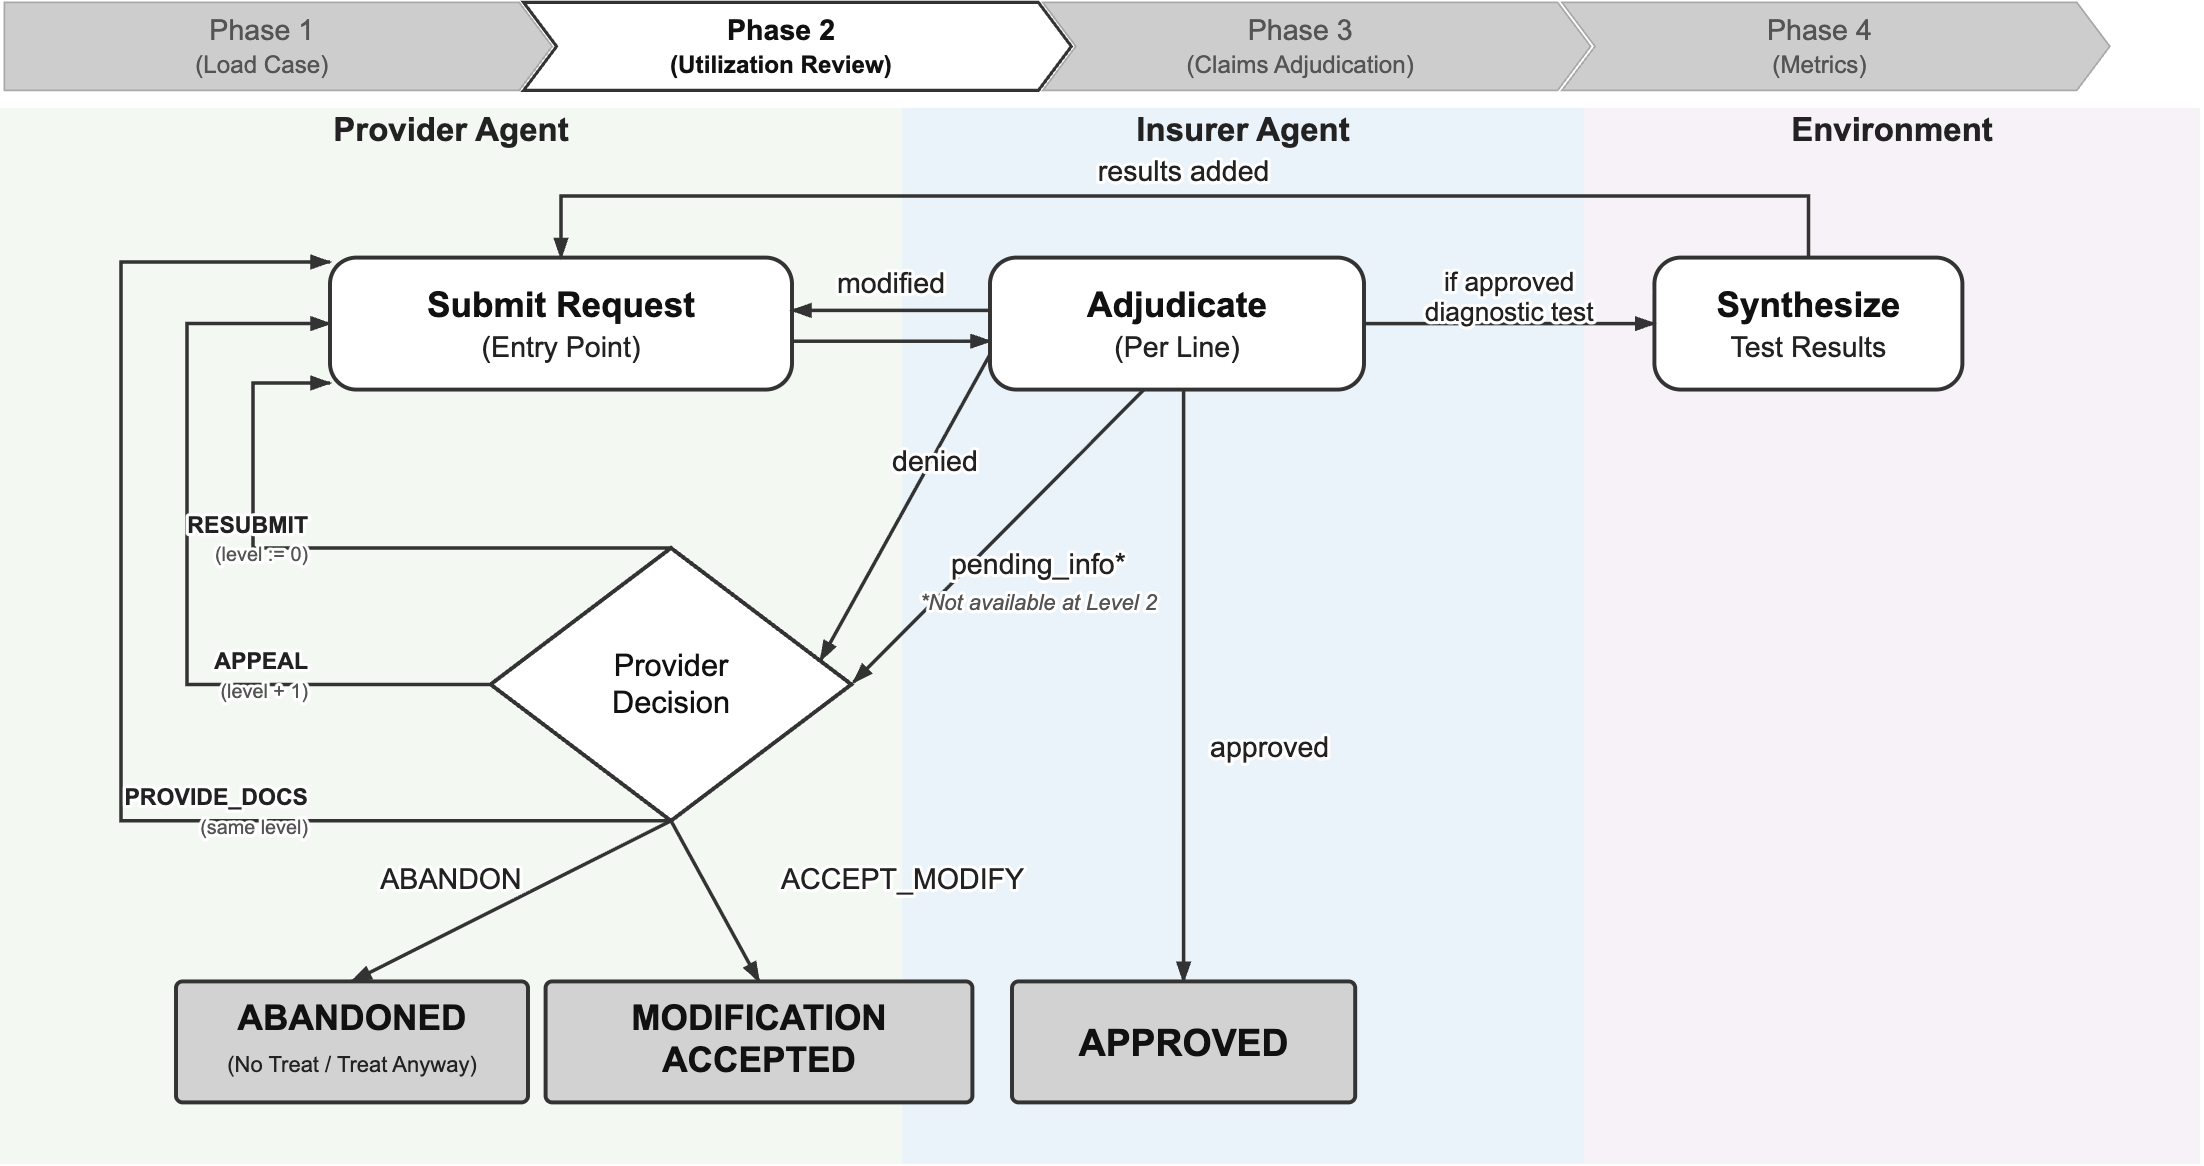
\includegraphics[width=\textwidth]{flowchart.png}
\caption{Phase~2 (Utilization Review) simulation flow. In utilization review, the provider seeks advance approval for planned services. Phase~3 (Claims Adjudication) follows the same structure but applies to services already delivered, with \texttt{WRITE\_OFF} (absorbing the unreimbursed cost) replacing the \texttt{ABANDON} actions. Full agent specifications are in Appendix~\ref{sec:agent-details}.}
\label{fig:flowchart}
\end{figure*}

The simulation proceeds in four phases (Figure~\ref{fig:flowchart}). Phase~1 presents the patient case to both agents with identical clinical facts. Phase~2 (Utilization Review) and Phase~3 (Claims Adjudication) contain the strategic interaction. Phase~4 computes the financial settlement, tallying reimbursement for each approved service line.

In Phase~2, the provider and insurer negotiate over prior authorization through alternating submissions and adjudications. The provider requests services with clinical justification; the insurer evaluates each request against coverage policy. When the insurer approves a laboratory or imaging order, the Environment module returns results drawn from the patient record. If no result exists in the source data for that test, the Environment generates a clinically plausible one, allowing the provider to incorporate new diagnostic findings into subsequent requests. Phase~2 continues until every requested service reaches a terminal state. Phase~3 follows the same logic but only for services that were approved or that the provider chose to deliver despite denial.

\begin{figure*}[t]
\centering
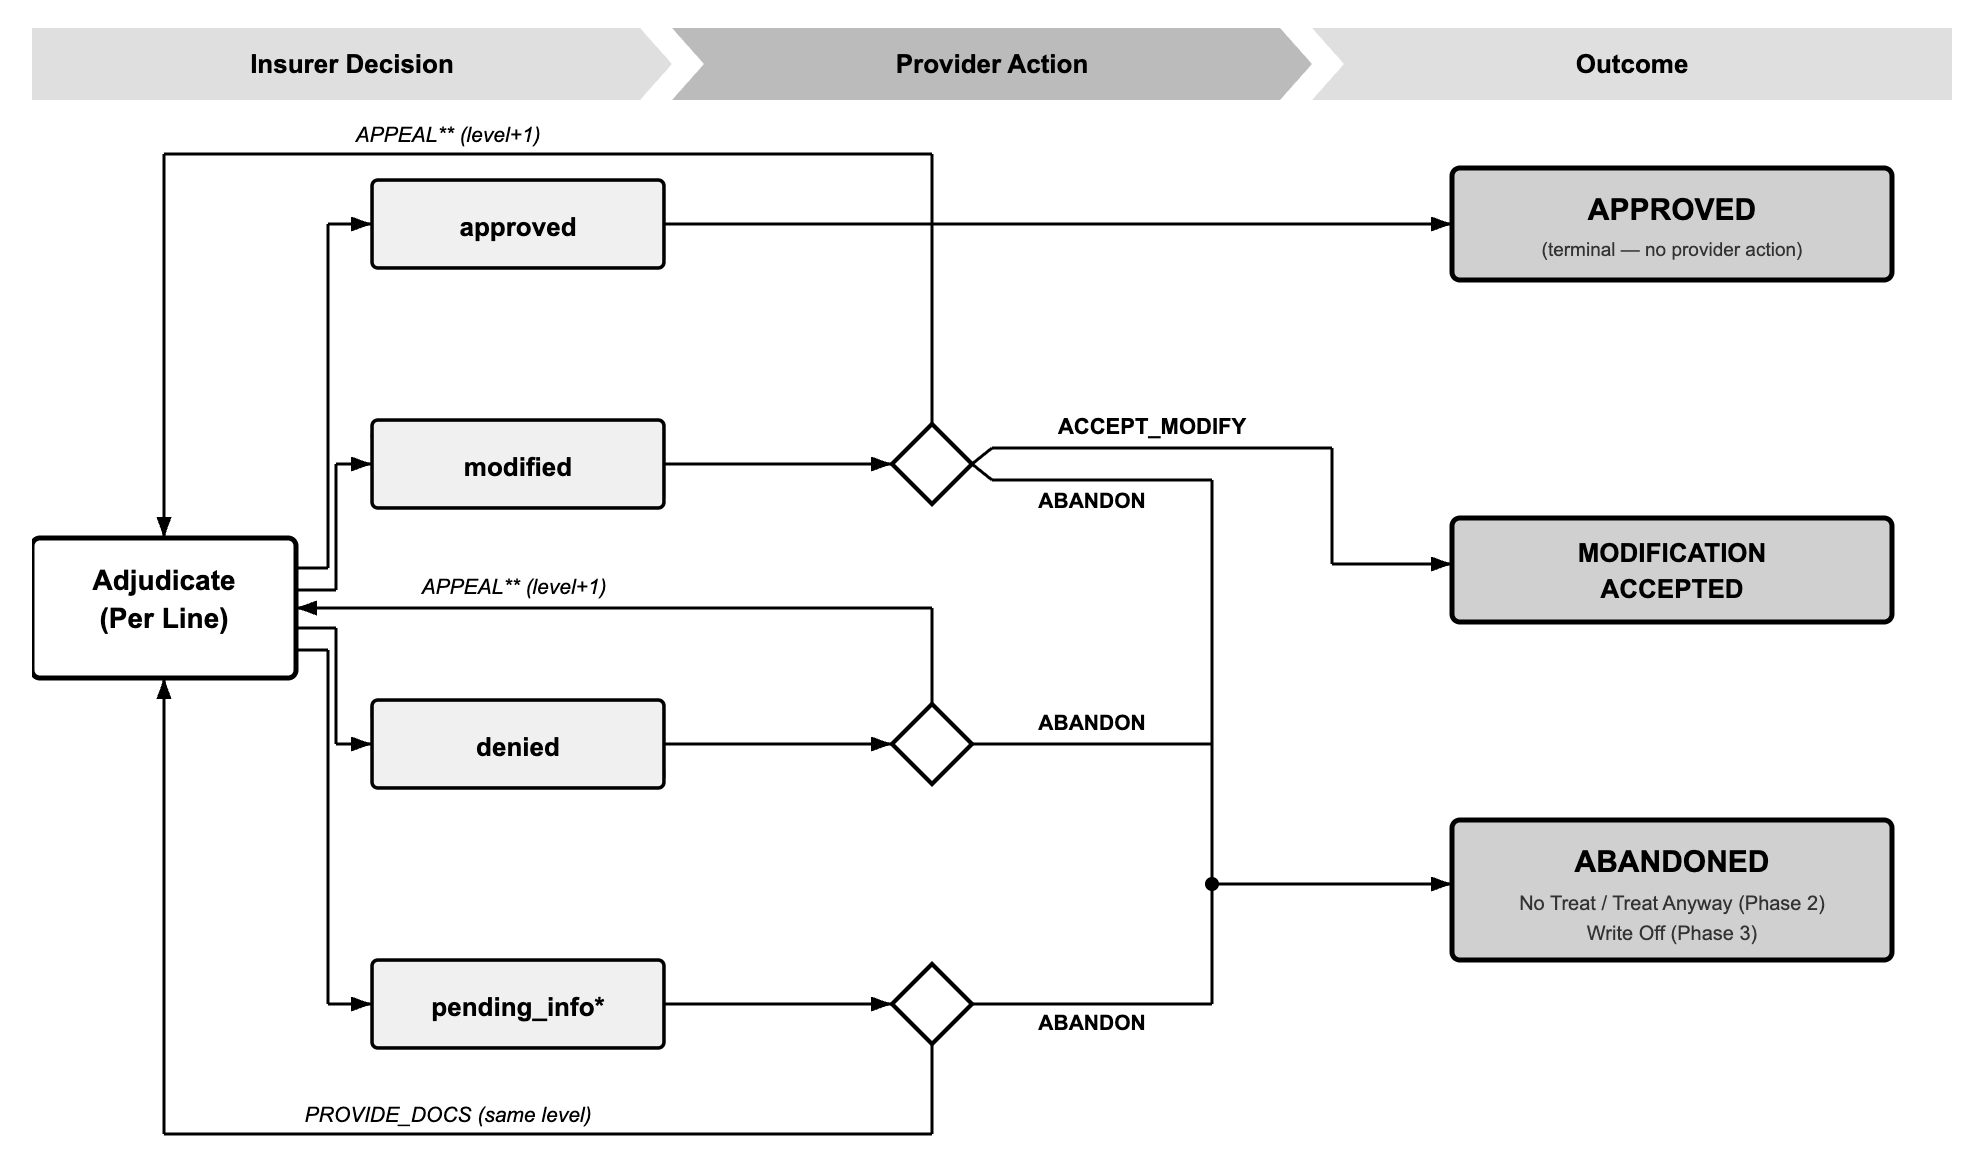
\includegraphics[width=\textwidth]{flowchart_2.png}
\caption{Provider per-line action space, expanding the provider decision node in Figure~\ref{fig:flowchart}. At any point the provider may also RESUBMIT (bundle-level), withdrawing all lines and restarting at Level~0 (see Figure~\ref{fig:flowchart}). *~pending\_info is not issued by the insurer at Level~2. **~APPEAL is not available at Level~2 (maximum review level). }
\label{fig:provider-action}
\end{figure*}

We model three review levels, grounded in the Medicare appeal structure \citep{cms2024appeals}: initial determination (Level~0), first-level appeal to a medical director (Level~1), and independent external review by a third party (Level~2). The simulation terminates at Level~2 because these three levels encompass the purely administrative prior authorization process, the domain where AI-driven automation is currently being deployed by both providers and insurers. Further legal appeals (e.g., Administrative Law Judge hearings and federal court proceedings) involve formal evidentiary rules and judicial oversight, placing them outside the scope of AI-mediated negotiation. Appendix~\ref{sec:appeal-levels} maps these to Medicare's five-level system.

\subsection{Strategy Operationalization}
\label{sec:strategy}

We operationalize three strategy conditions that govern how each agent resolves interpretive ambiguity in the gray zone. In the \textbf{default} condition, no strategy guidance is added to the agent's prompt, revealing the LLM's baseline behavior when faced with ambiguous policy interpretation. In the \textbf{cooperate} and \textbf{defect} conditions, we add interpretive guidance to the system prompt. The cooperate and defect prompts are designed to be symmetric: each resolves the same ambiguity in opposite directions without altering the underlying clinical facts or policy criteria. All conditions share the same clinical facts, clinical guideline, and coverage policy; they differ only in ambiguity-resolution framing:

\textbf{Provider cooperate:} ``Choose the minimum clinically defensible set of requested services and the lowest reasonable intensity that still supports timely, appropriate treatment.''

\textbf{Provider defect:} ``Choose the maximum plausibly defensible set of requested services and the highest plausible intensity supported by the case facts and policy. Include additional supportive line items (e.g., extra diagnostics, monitoring) if remotely justifiable; do not fabricate clinical facts.''

\textbf{Insurer cooperate:} ``Apply policy in a good-faith, access-preserving way. If the request plausibly satisfies policy, approve. Prefer approve over deny when policy interpretation is genuinely ambiguous.''

\textbf{Insurer defect:} ``Apply policy in a strict, cost-containment way. If the request is not clearly supported by explicit policy criteria and documentation, deny or modify/downgrade. Prefer deny over approve when evidence is borderline.''

Full prompts are provided in Appendix~\ref{sec:prompts}.

\subsection{Experimental Design}
\label{sec:design}

We employ a 3$\times$3 full factorial design, crossing three provider strategies (cooperate, defect, default) with three insurer strategies (cooperate, defect, default), yielding nine experimental conditions (Table~\ref{tab:conditions}).

\begin{table*}[h]
\centering
\caption{Experimental conditions. Condition labels encode provider strategy (first letter: C = Cooperate, D = Defect, N = Default) and insurer strategy (second letter after underscore). For example, CP\_DI denotes a cooperating provider against a defecting insurer.}
\label{tab:conditions}
\begin{tabular}{lccc}
\toprule
 & \textbf{Insurer C} & \textbf{Insurer D} & \textbf{Insurer N} \\
\midrule
\textbf{Provider C} & CP\_CI & CP\_DI & CP\_NI \\
\textbf{Provider D} & DP\_CI & DP\_DI & DP\_NI \\
\textbf{Provider N} & NP\_CI & NP\_DI & NP\_NI \\
\bottomrule
\end{tabular}
\end{table*}
